\documentclass{article}

\usepackage{fancyhdr}
\usepackage{extramarks}
\usepackage{amsmath}
\usepackage{amsthm}
\usepackage{amsfonts}
\usepackage{tikz}
\usepackage[plain]{algorithm}
\usepackage{algpseudocode}

\usetikzlibrary{automata,positioning}

%
% Basic Document Settings
%

\topmargin=-0.45in
\evensidemargin=0in
\oddsidemargin=0in
\textwidth=6.5in
\textheight=9.0in
\headsep=0.25in

\linespread{1.1}

\pagestyle{fancy}
\lhead{\hmwkGroupName}
\chead{\hmwkClass\ : \hmwkTitle}
\rhead{\firstxmark}
\lfoot{\lastxmark}
\cfoot{\thepage}

\renewcommand\headrulewidth{0.4pt}
\renewcommand\footrulewidth{0.4pt}

\setlength\parindent{0pt}

%
% Create Section Headers
%

\newcommand{\startSectionHeader}[1]{
\nobreak\extramarks{#1}{}\nobreak{}
}

\newcommand{\enterSectionHeader}[1]{
    \nobreak\extramarks{}{#1 continued on next page\ldots}\nobreak{}
    \nobreak\extramarks{#1 (continued)}{#1 continued on next page\ldots}\nobreak{}
}

\newcommand{\exitSectionHeader}[0]{
\nobreak\extramarks{\currentSectionName (continued)}{\currentSectionName continued on next page\ldots}\nobreak{}
\nobreak\extramarks{\currentSectionName}{}\nobreak{}
}

\setcounter{secnumdepth}{0}

%
% Homework Problem Environment
%

\newenvironment{homeworkProblem}{
\section{\currentSectionName}
\enterSectionHeader{\currentSectionName}
}{
\exitSectionHeader{}
}


%
% Homework Details
%   - Title
%   - Class
%   - Author
%

\newcommand{\hmwkTitle}{Term Project - Rollercoasters}
\newcommand{\hmwkClass}{MATH2850J}
\newcommand{\hmwkAuthor}{Guo shitong Ren zhixing Wang qingyu Yuan yilei Zhang kangqi}
\newcommand{\hmwkDate}{\today}
\newcommand{\hmwkGroupName}{\textbf{Group 14}}

%
% Title Page
%

\title{
    \vspace{2in}
    \textmd{\textbf{\hmwkTitle}}\\
    \vspace{3in}
}
\author{\hmwkAuthor}
\date{\hmwkDate}


\renewcommand{\part}[1]{\textbf{\large Part \Alph{partCounter}}\stepcounter{partCounter}\\}

% Alias for the Solution section header
\newcommand{\solution}{\textbf{\large Solution}}

\begin{document}

\maketitle

\pagebreak
\nobreak\extramarks{Contents}{}\nobreak{}
\tableofcontents

\pagebreak
\newcommand{\currentSectionName}{Abstract}
\startSectionHeader{\currentSectionName}
\begin{homeworkProblem}
In this study, we mainly focus on two aspects of roller coaster research, namely the impact of track shape on passengers' experience and the impact of seating position on passengers' experience. In brief, we first focus on comparing and analyzing the pros and cons of various roller coaster models, and we simplify various realistic shapes into different curve models in mathematics for analysis. Combining mathematical formulas and physical principles, we try to find a type of ideal roller coaster that can give people a sense of both thrill and comfort, that is to say, to avoid the situation where the roller coaster will experience a sudden change in G-force when it enters a circular track from a flat track. Based on this problem, we analyze and calculate three models, namely circular track, the one that can provide constant G-force and Cornu spirals. Thus we find that the first model cannot solve the existing problem, the second model can provide constant G-force during the roller coaster’s journey, but still cannot solve the problem of sudden change at the beginning and end. Cornu spirals can provide g acceleration at the beginning and end, which is consistent with the acceleration of the roller coaster on a flat track, and it is a very smooth curve because it has a high derivative. Further, if we want to design a roller coaster model that is safe and comfortable throughout the journey, we can consider combining the bottom of Cornu spirals with the upper part of the model that can provide constant G-force, thus obtaining a constant G-force throughout the journey and no sudden change in G-force at the beginning and  the  end.If we want to design a thrilling and comfortable one. On the other hand, we study the impact of seating position on passenger experience on a circular vertical loop. We found that compared with passengers sitting in the middle, passengers sitting in the front and back feel more obvious, that is, more stimulating.
\end{homeworkProblem}

\renewcommand{\currentSectionName}{Introduction}
\startSectionHeader{\currentSectionName}
\pagebreak
\begin{homeworkProblem}
\subsection{Introduction of circular vertical loops}
    The track of the Flip Flap Railway is a perfect circle. The radius of it is $R$.

    The net force is $\frac{mv^2}{r}$, where $r$ is the radius of curvature, which is the reciprocal of curvature.

    For
    $
        \varphi(t) =
        \begin{pmatrix}
            R\cos t \\
            R\sin t
        \end{pmatrix}
    $,
    we have

    $$
        \varphi'(t) =
        \begin{pmatrix}
            -R\sin t \\
            R\cos t
        \end{pmatrix},\
        T\circ\varphi(t) =
        \begin{pmatrix}
            -\sin t \\
            \cos t
        \end{pmatrix},\
        (T\circ\varphi)(t) =
        \begin{pmatrix}
            -\cos t \\
            -\sin t
        \end{pmatrix}
    $$

    By substituting the quantities, we obtain

    $$
        \kappa=\frac{||(T\circ\varphi)'(t)||}{||\varphi'(t)||}=\frac{1}{R},
    $$

    which indicates that the radius of the curvature is a constant $R$.

    Thus, when the Flip Flap Railway reaches the lowest position, the normal force reaches max, which is:

    \begin{equation}
        N=\frac{mv_{\mathrm{bottom}}^2}{R}+mg.
    \end{equation}

    Since it's weightless at the top, we have

    \begin{equation}
        \frac{mv_{\mathrm{top}}^2}{R}=mg.
    \end{equation}

    Thus,

    $$
        v_{\mathrm{top}}=\sqrt{gR}.
    $$

    Supposing that there is no friction, by the conservation of mechanical energy, we have

    \begin{equation}
        \frac{1}{2}mv_{\mathrm{bottom}}^2=mgh+\frac{1}{2}mv_{\mathrm{top}}^2
    \end{equation}
\subsection{Disadvantageous of circular loops}
    Combining Eq.(1)(2)(3), we obtain

    $$
        N=6mg=6G_s.
    $$


    When entering the loop, the $G$-force suddenly acts on the passengers whose maximum value is $6G_s$.However,in \cite{ref4} the author states that the general audience can't bear $6g$ for for any extended time.Hence,such design will take a toll on passengers' physical health.

    (In \cite{ref1}, the author states that the maximum $G$-force can reach 12$G_s$. It's not the condition of a perfect circle. Instead, it is possible for a curve with the curvature becomes larger in the process of from top to bottom.)



\pagebreak


\indent{Some alternative vertical loops: }
We can see from above that,since the sudden change of G-force will have a negative impact on people's health and it can't meet the needs of both thrilling and comfortable,the circular roller coaster loop has been replaced with some other alternative vertical loops.Some of them are designed to offer constant centripetal acceleration,and the others are designed to offer constant G-force.But both of them can' get rid of the disadvantageous of the sudden change of  G-force at the beginning and the end.So,the designers come up with the Cornu spiral model.\\
\subsection{Introduction of Cornu spirals }
\subsubsection{The definition of Cornu spirals}
The Fresnel Integrals,known as $C(t)$ and $S(t)$,where
$$
C(t)=\int_{0}^{t}cos(\frac{\pi}{2}s^2)ds
$$
$$
S(t)=\int_{0}^{t}sin(\frac{\pi}{2}s^2)ds
$$
Then, the Cornu spiral can be parametrized by:
$$
x(s)=C(\sqrt{\frac{2s}{\pi}})
$$
$$
y(s)=S(\sqrt{\frac{2s}{\pi}})
$$
\begin{figure}[H]
        \centering
        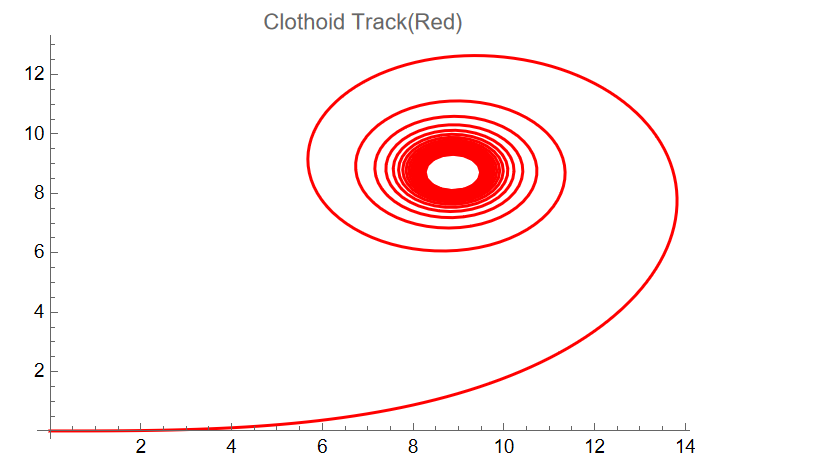
\includegraphics[width=0.4\textwidth]{clothoid.png}
        \label{1}
        \caption{The Cornu spiral}
    \end{figure}
\subsubsection{Properties of Cornu spirals }

    To find the radius of curvature, we need to find the curvature, which is given by:
\begin{equation}
\kappa(s) &= \frac{x’(s)y’’(s) - x’’(s)y’(s)}{(x’(s)^2 + y’(s)^2)^{3/2}}
    \end{equation}  
    where x’(s), x’’(s), y’(s), \text{ and } y’’(s) \text{ are the first and second derivatives of } x(s) \text{ and } y(s) \text{ with respect to } s.\ \
To find these derivatives, we need to use the chain rule and the properties of the Fresnel integrals. We have
$$x’(s) &= \frac{d}{ds} C\left(\sqrt{\frac{2s}{\pi}}\right) = \frac{1}{2} \sqrt{\frac{2}{\pi s}} C’\left(\sqrt{\frac{2s}{\pi}}\right) = \sqrt{\frac{1}{\pi s}} \cos \frac{s}{\pi}$$
where we use 
$$
C’(t) = \cos \frac{\pi t^2}{2}
$$
Similarly, we have
$$
y’(s) &= \sqrt{\frac{1}{\pi s}} \sin \frac{s}{\pi}
$$
where we use 
$$
S’(t) = \sin \frac{\pi t^2}{2}
$$
For the second derivatives, we have
$$ x’’(s) &= -\frac{1}{4} \sqrt{\frac{1}{\pi s^3}} (\cos \frac{s}{\pi} + 2 s \sin \frac{s}{\pi})$$
Similarly, we have
$$ y’’(s) &= -\frac{1}{4} \sqrt{\frac{1}{\pi s^3}} (\sin \frac{s}{\pi} - 2 s \cos \frac{s}{\pi})$$

Then,we plug these derivatives into the formula for curvature and simplify it ,and finally we get  the radius of curvature is inversely proportional to the distance s from the center.
\subsubsection{Advantageous from mathematical perspective}
From the mathematical perspective,the sudden change of G-force can be interpreted as an immediate transition from one radius of curvature to another,which will give a
continuous, smooth track, but with discontinuous second derivatives. \cite{ref1}So,to tackle these problem,we should make the curve  smoother and smoother.We know that a curve with a parametrization  whose second derivatives are continuous,is considered to be smoother than the one with a parametrization  whose second derivatives are discontinuous.\\
Then,we can see from above that the first derivatives and the second derivatives are both continuous because they are the results of the elementary of some simple continuous functions.To be more general,since the Cornu spiral can be expressed using continuous and differentiable functions sine and cosine, it is infinitely differentiable ,meaning quite high derivatives.\\

\subsubsection{Advantageous from  physics perspective}
By applying the Cornu spirals model,we can adjust the G-forces by scaling.We know that we can obtain G-force by
\begin{equation}
    m\frac{v^2}{R}=N-mgcos(\theta)
\end{equation}
So,G-force can be expressed as
\begin{equation}
    G=\frac{N}{mg}=\frac{v^2}{Rg}+cos(\theta)
\end{equation}
And also,according to the Conservation of energy Law
\begin{equation}
    v^2-v_{0}^2=2gh
\end{equation}
Finally,G-force can be expressed as 
\begin{equation}
    G=\frac{v_{0}^2}{rg}+\frac{2h}{R}+cos(\theta)
\end{equation}
where $v_{0}$ is the initial velocity,$h$ is the instant height,and $\theta$ is the instant angle between the vertical line and the position.\\
Using the parametrization of The Fresnel Integrals,we know that $y(s)$ can be seen as $h$ here,and $\frac{y(s)}{\sqrt{x^2(s)+y^2(s)}}$ equals to $cos(\theta)$ here.So,we can plot the curve using mathematica.,which can be seen in Figure \ref{3}
\begin{figure}[H]
        \centering
        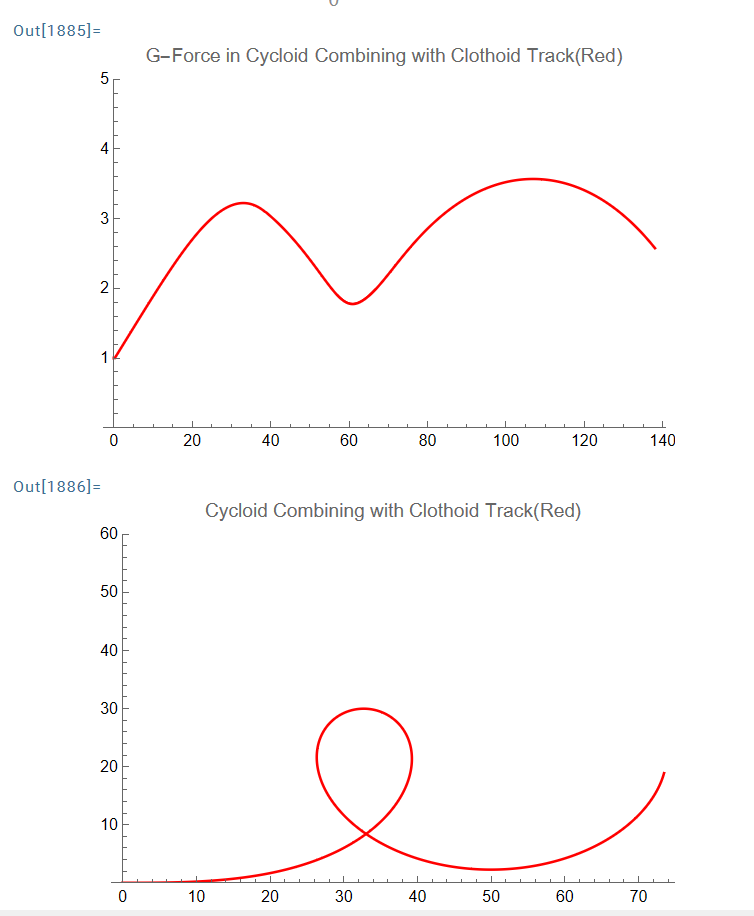
\includegraphics[width=0.4\textwidth]{clothoid_model.png}
        \label{3}
        \caption{The Cornu spiral model}
    \end{figure}
Regardless of the  scalar factor,the G-force at the beginning and the end of the loop is found to be always equal to exactly 1g,which means there won't be a sudden change on G-force when the train enters and exits the vertical loop.\\

\end{homeworkProblem}

\renewcommand{\currentSectionName}{Analysis}
\startSectionHeader{\currentSectionName}
\pagebreak
\begin{homeworkProblem}
\subsection{Analysis of the difference in G-force among different positions}
Since the roller coaster is a whole, the position of each person relative to the coaster as a whole can be approximated as a prime point.
We can reduce a roller coaster to a rope of uniform mass whose internal tension can be varied to maintain a particular shape of the rope.\\
Suppose the mass of a unit length is $\rho$. The whole length of the roller coaster is R$\phi$.
\\Since geometrical relation:
$$
\mathrm{d}l= R\mathrm{d}\theta\ 
$$
\\where $\theta$ is the angle between the line joining the microelement and the center of the circle and the vertical line
Hence, the mass of a small segment of microelements
$$
        \mathrm{d}m=\rho R\mathrm{d}\theta
        $$
\\ The moment of inertia of the rope can be shown as:
$$
I =\int  R^2 \cdot dm = R^3\rho\phi.
$$
where
    $$
    \phi_1+\phi_2=\phi=\mathrm{const}.
    $$

$\phi_1$ is the angle between the line joining the apex of the left end of the rope and the center of the circle and the vertical line
\\$\phi_2$ is the angle between the line joining the apex of the right end of the rope and the center of the circle and the vertical line
\\If there is no friction force, by energy conservation:

    $$
    E=\rho R\phi R(1-\cos\varphi)+\frac{1}{2}\rho R^3\phi\dot{\theta}^2
    $$

    $$
    E=\rho R\phi R(1-\cos(\phi_2-\frac{\phi}{2}))+\frac{1}{2}\rho R^3\phi\dot{\phi_2}^2
    $$
    According to the angular momentum theorem, $ \frac{dL}{dt}=\tau_{ext}$
$$ I\frac{d\theta}{dt}=\tau_{ext}$$
    $$
    -\rho\phi Rg^2\sin(\phi_2-\frac{\phi}{2})=\rho R^3\phi\ddot{\phi}_2
    $$

    $$
    \ddot{\phi}_2=-\frac{g}{R}\sin(\phi_2-\frac{\phi}{2})
    $$

    
    Now, do a force analysis on the dm microelement.
    \\ Normal phase forces are balanced, and hence we get:
    $$
    T\mathrm{d}\theta+N+\mathrm{d}mg\cos\theta=\mathrm{d}m\omega^2r
    $$
    \\Take a frame of reference with angular accelerating counter-clockwise:
\\We have compensated inertia force: $F=-m \ddot{\phi}_2 R$
    \\ tangential phase forces are balanced, and hence we get:
    $$
   \mathrm{d}T=g\sin\theta\mathrm{d}m + \mathrm{d} F
    $$
   $$
    \Rightarrow\mathrm{d}T=\rho Rg\sin\theta\mathrm{d}\theta+\underbrace{\rho gR\sin(\phi_2-\frac{\phi}{2})}_{\mathrm{constant}}\mathrm{d}\theta
    $$
With boundary equation:
    $$
    T|_{\phi_2}=T|_{\phi_1}=0
    $$
Therefore, we can get the relation between $\theta$ and $T$
    \begin{equation}
        T(\theta)=\rho gR(\cos{\phi_2}-\cos\theta)+\rho gR\sin(\phi_2-\frac{\phi}{2})(\phi_2-\theta)
    \end{equation}
Hence,
    \begin{equation}
G-Froce_s=a_{people feel}=\frac{N}{\mathrm{d}m}=\omega^2r-g\cos\theta-T\frac{\mathrm{d}\theta}{\mathrm{d}m}=\omega^2r-g\cos\theta-\frac{T}{\rho R}
    \end{equation}

    \begin{enumerate}

        \item[\textbf{Case 1:}] 
The leftmost passenger is at the apex.
        $\theta=0,\phi_1=0,\phi_2=\phi,T\approx 0$.
        
        \item[\textbf{Case 2:}] 
The rightmost passenger is at the apex.
        $\theta=0,\phi_1=\phi,\phi_2=0,T\approx 0$.

        \item[\textbf{Case 3:}] 
The middle passenger is at the apex.
        $\theta=0,\phi_1=\frac{\phi}{2},\phi_2=\frac{\phi}{2},T\approx \rho gR(\cos\frac{\phi}{2}-1)$.

        Substituting Eq.(2) into the equation above, we have

        $$
a_{left}=a_{right}=\omega^2_{\mathrm{side top}}r-g\cos{\frac{\phi}{2}-\frac{\phi}{2}}=\omega^2_{\mathrm{side top}}R-g
        $$

        $$
\Delta \omega^2=\omega^2_{\mathrm{side top}}-\omega^2_{\mathrm{middle top}}=\frac{2g}{R}(1-\cos\frac{\phi}{2})
        $$

        $$
a_{middle}=\omega^2_{\mathrm{side top}}r-\Delta \omega^2r-g\cos\frac{\phi}{2}
        $$
$$ =\omega^2_{\mathrm{side top}}r-2g(1-\cos\frac{\phi}{2})-g\cos\frac{\phi}{2}=\omega^2_{\mathrm{side top}}R-2g+g\cos\frac{\phi}{2}$$
$$<\omega^2_{\mathrm{side top}}R-g =a_{left}=a_{right}$$
So the accelerate of the two sides is larger than that of the middle.
\end{enumerate}

\end{homeworkProblem}

\renewcommand{\currentSectionName}{Verification}
\startSectionHeader{\currentSectionName}
\pagebreak
\begin{homeworkProblem}
\subsection{Theorem analysis}
Constant G-force rollercoasters are those providing the constant normal force during the process. There's a previous article \cite{ref1} that has conducted the numerical calculations for constant G-force rollercoasters and got some graphs. However, the detailed calculation process is not performed. Thus, the verification done by Mathematica follows.


During the process, the centripetal acceleration $a$ is expressed as:
    \begin{equation}
    a=\frac{v^2}{R},
    \end{equation}
where $v$ is the velocity, and $R$ is the radius at that moment. Meanwhile, the relation between centripetal acceleration and the constant acceleration provided by the normal force is expressed as:
    \begin{equation}
    a=a_{n}-g cos{\theta},
    \end{equation}
where $a$ is the centripetal acceleration, $a_n$ is the acceleration provided by the normal force, $g$ is the gravity, and $\theta$ is the angle between the normal force and the gravity.
Then, by applying conservation of mechanical energy to the process, we have
    \begin{equation}
    \frac{1}{2} m {v_{0}}^2=m g h + \frac{1}{2} m {v_{1}}^2,
    \end{equation}
where $m$ is the mass of the object, $v_0$ is the initial velocity, $h$ is the height of a arbitrary moment, and $v_1$ is the velocity at the moment with the height $h$. Combining Eq.(1) (2) (3) together, we have
    \begin{equation}
    R=\frac{{v_0}^2-2gh}{a_n-g \cos{\theta}}
    \end{equation}

Next, we use Mathematica to verify the shape of the constant G-force rollercoaster track. The theorem is the differential on arc. For a tiny arc, the change of curvature can be neglected, namely the radius is the same as shown in the picture.

\begin{figure}[htbp]
    \centering
    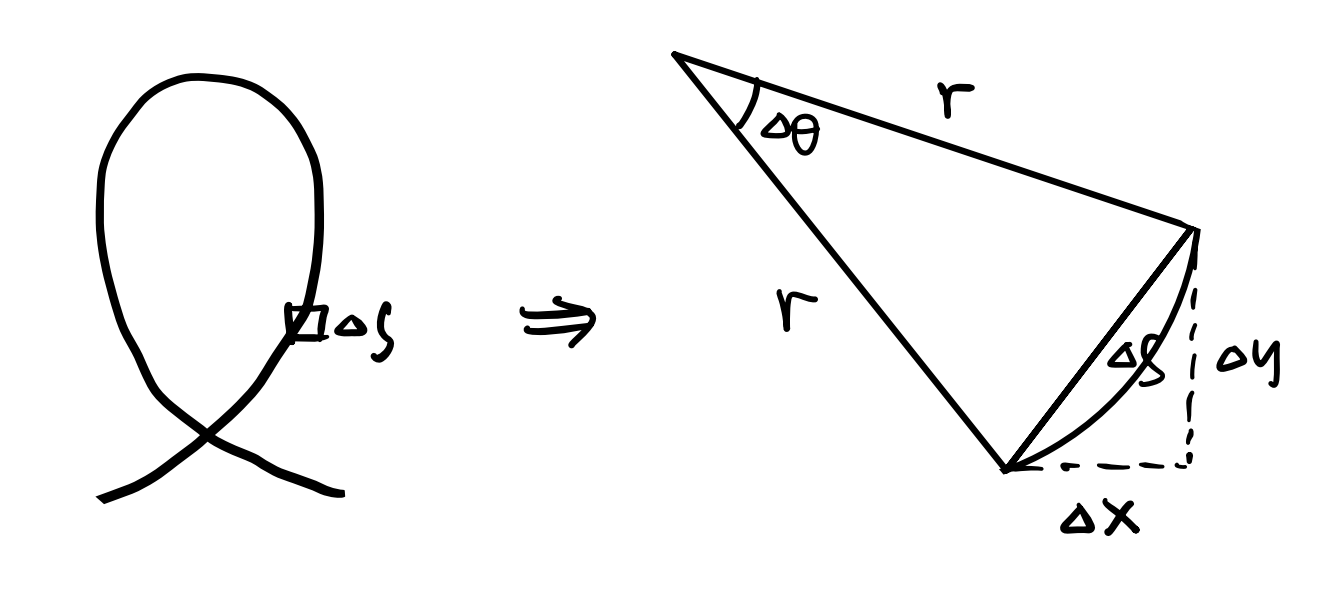
\includegraphics[width=0.4\textwidth]{1.png}
    \caption{Arc Differential}
    \end{figure}  

The relation between the small radius $\theta$ and small arc length $s$ is expressed as:
    \begin{equation}
    \Delta s=r\Delta \theta.
    \end{equation}
Combining the change in x-component, $dx$, and y-component, $dy$, of the arc, we have a series of differential equations.

$$ \left\{
\begin{aligned}
\frac{\partial \theta}{\partial s} & = \frac{1}{r} \\
\frac{\partial x}{\partial s} & =  \cos \theta \\
\frac{\partial y}{\partial s} & =  \sin \theta
\end{aligned}
\right.
$$
Applying Euler's Method, we have

$$ \left\{
\begin{aligned}
x_{n+1}=x_{n}+ \cos (\theta_{n})(s_{n+1}-s_{n}) \\
y_{n+1}=y_{n}+ \sin (\theta_{n})(s_{n+1}-s_{n}) \\
\end{aligned}
\right.
$$
With the help of the computing of Mathematica, we can find the shape of the track.

\subsection{Verification of constant G-force track non-friction condition}

For the initial value, we set the initial velocity to be $27m/s$, the gravity constant to be $9.81m/s^2$, and the constant G-force to be $35m/s^2$. The coding part of the non-friction condition follows, ,

\begin{figure}[H]
    \centering
    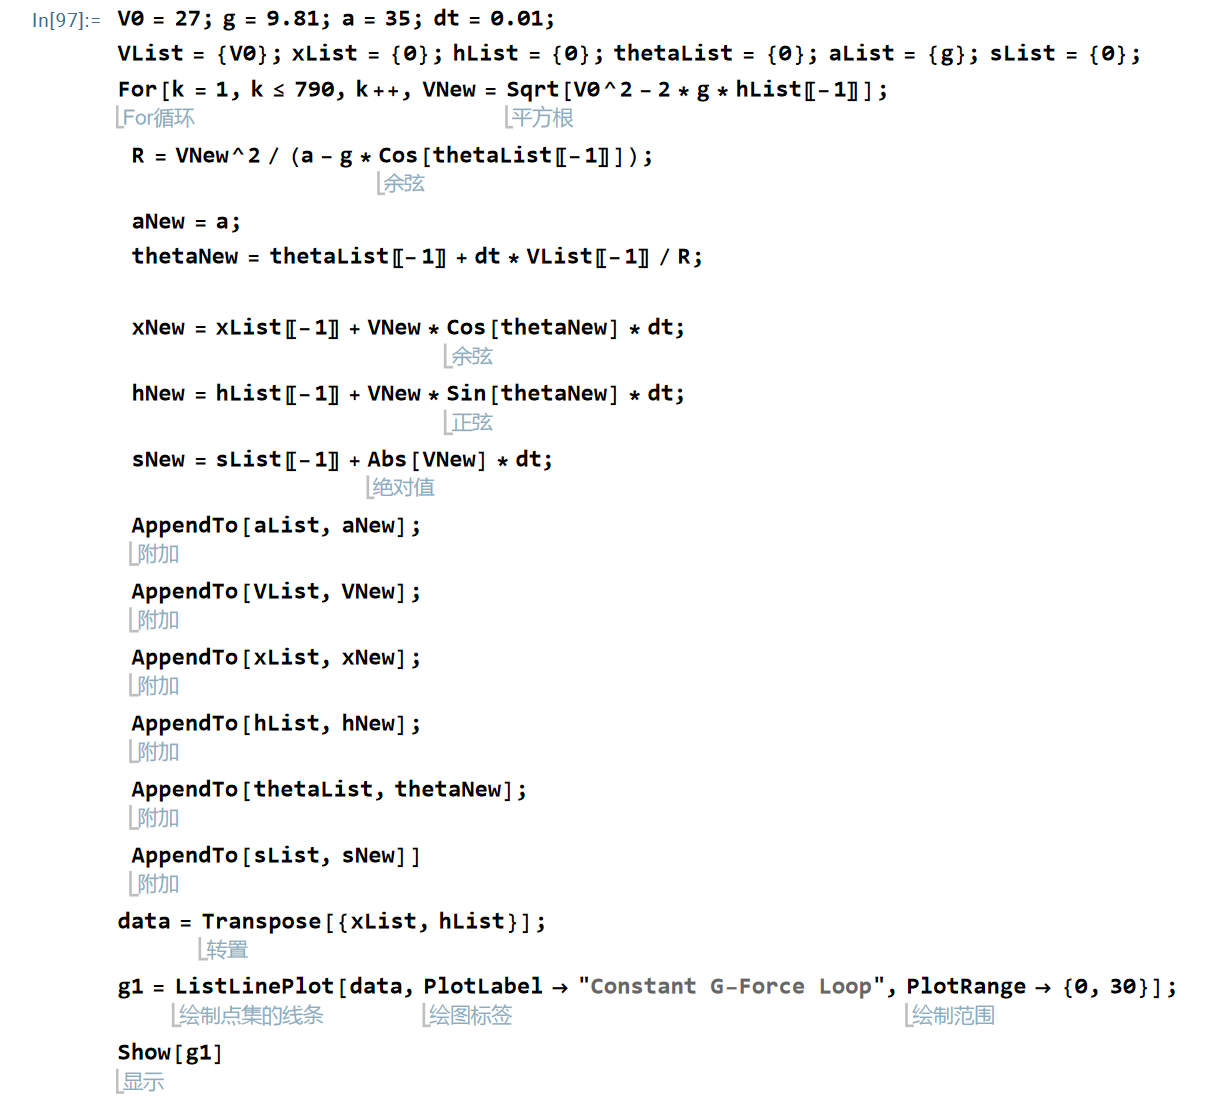
\includegraphics[width=0.6\textwidth]{2.png}
    \caption{Codes of Generating The Constant G-force Track Shape (Non-friction)}
    \end{figure}  


The result of graph follows, which is very close to the one in the article.

\begin{figure}[H]
    \centering
    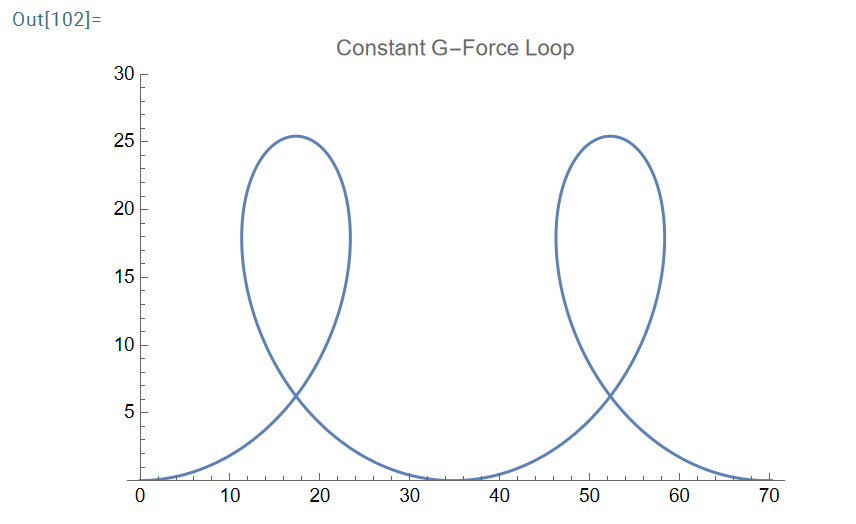
\includegraphics[width=0.4\textwidth]{3.png}
    \caption{The Constant G-force Track Shape (Non-friction)}
    \end{figure}  


\begin{figure}[H]
    \centering
    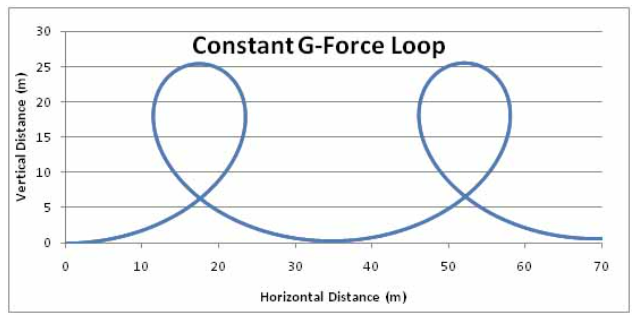
\includegraphics[width=0.4\textwidth]{4.png}
    \caption{The Constant G-force Track Shape in The Article (Non-friction)}
    \end{figure}  


\subsection{Verification of constant G-force track at friction condition}
Similarly, for the initial value, we set the initial velocity to be $27m/s$, the gravity constant to be $9.81m/s^2$, and the constant G-force to be $35m/s^2$. The coding part at the condition with friction follows,

\begin{figure}[H]
    \centering
    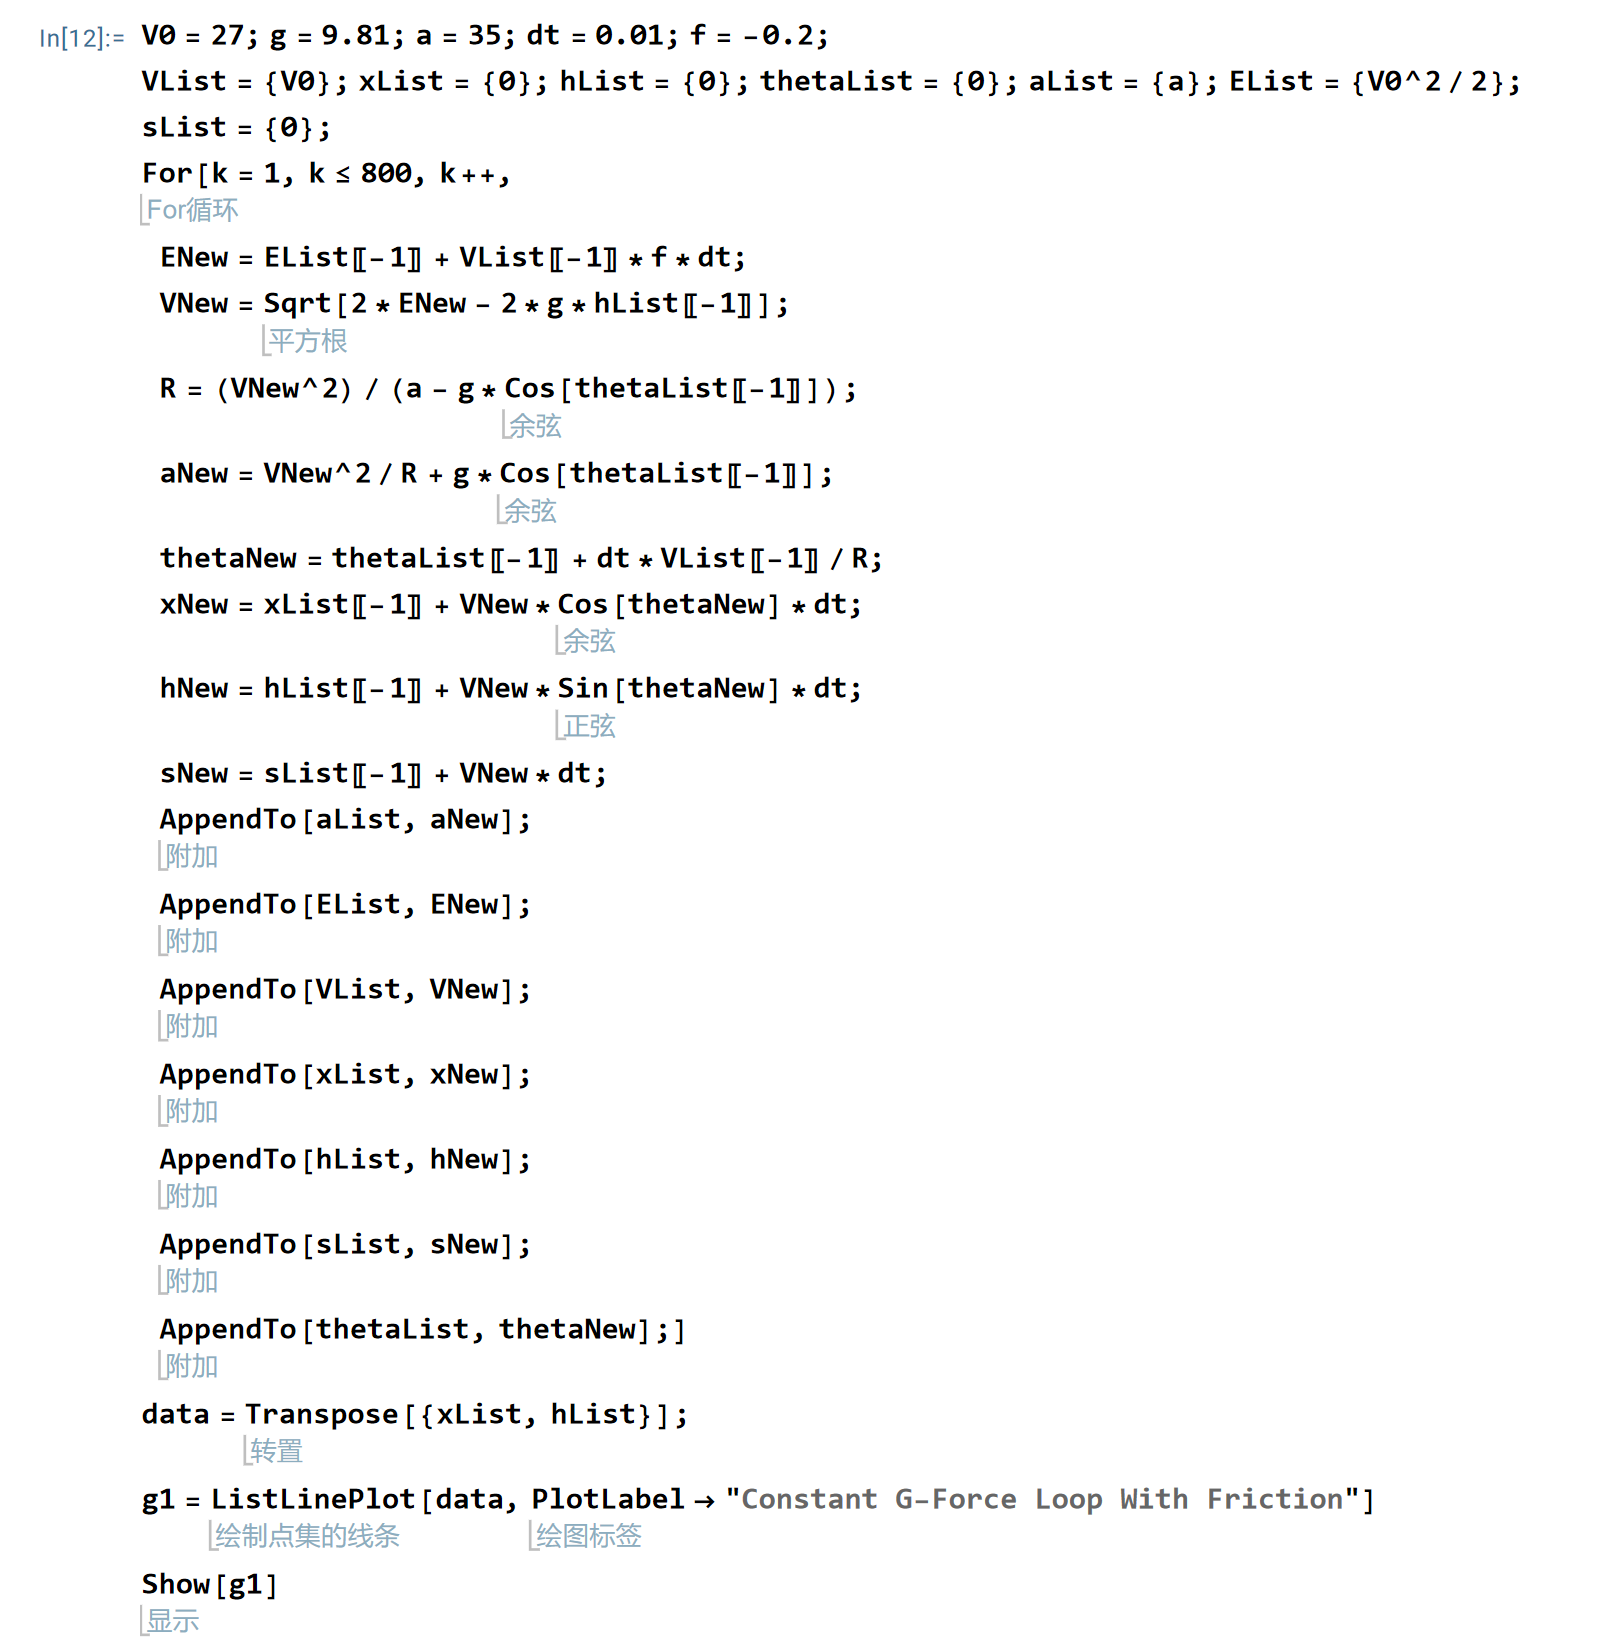
\includegraphics[width=0.6\textwidth]{5.png}
    \caption{Codes of Generating The Constant G-force Track Shape (With Friction)}
    \end{figure}  

The result of graph follows, which is also close to the one in the article and the shape of a real-life coaster, the “Great American Scream Machine” [5].

\begin{figure}[H]
    \centering
    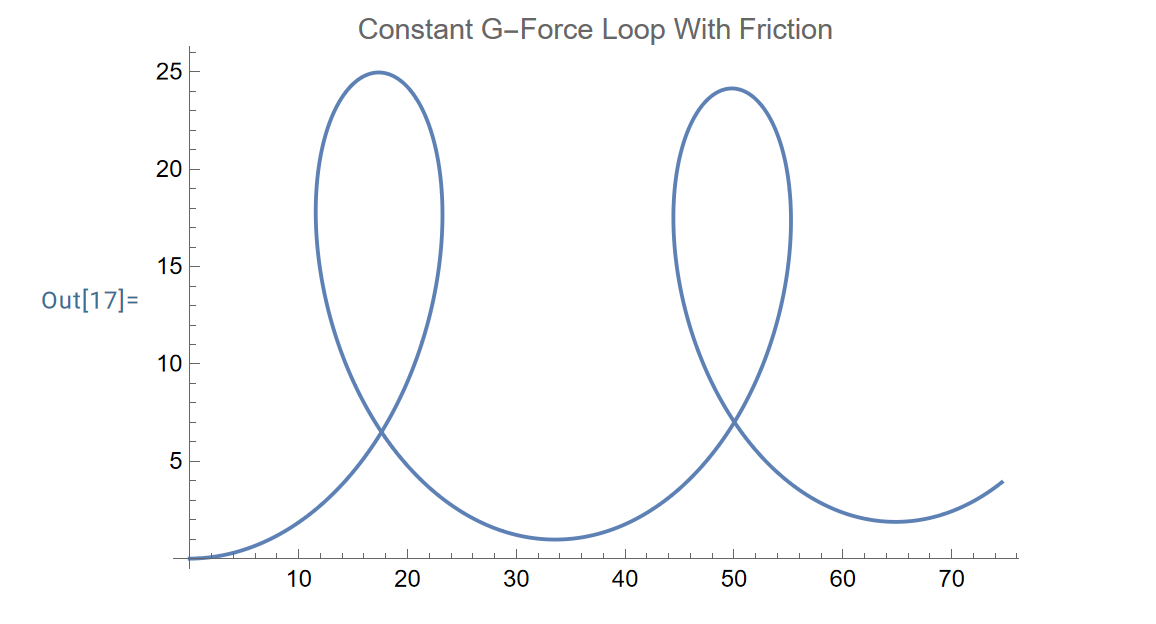
\includegraphics[width=0.4\textwidth]{6.png}
    \caption{The Constant G-force Track Shape (With Friction)}
    \end{figure}  
    
\begin{figure}[H]
    \centering
    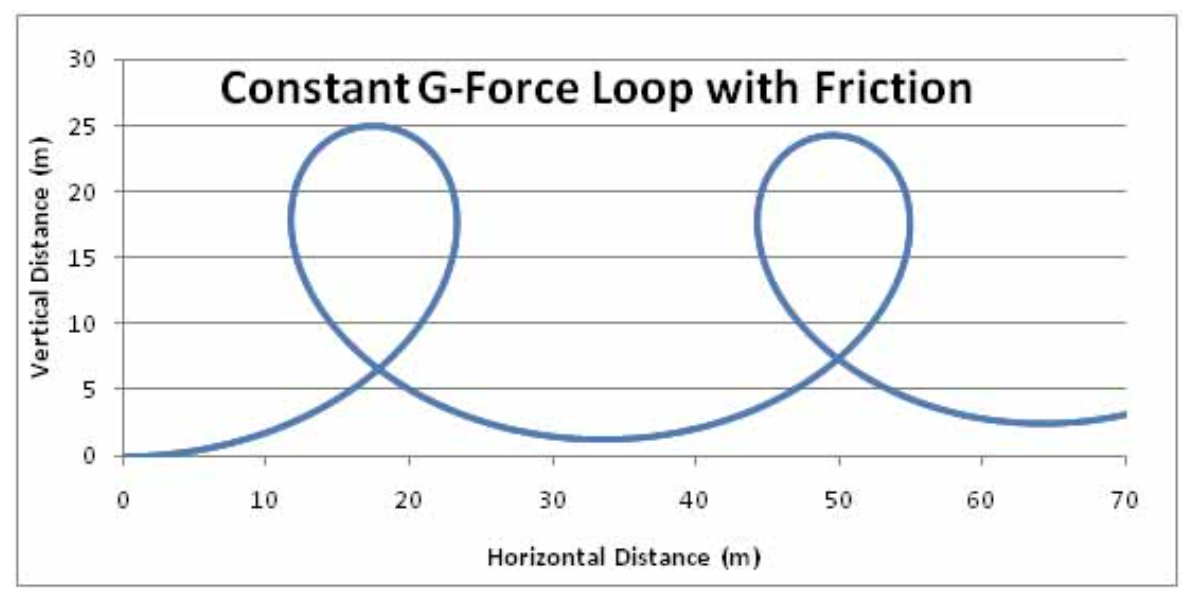
\includegraphics[width=0.4\textwidth]{7.png}
    \caption{The Constant G-force Track Shape in The Article (With Friction)}
    \end{figure}      
    
\subsection{Verification of cycloid track at non-friction condition}
The article also mentioned the generated shape of constant G-force rollercoaster track is similar to the shape of cycloid. The verification follows.

We first need to generate a cycloid that fits the track we found in Figure 5. The general expression for a cycloid is
$$ \left\{
\begin{aligned}
x & = at-b\sin t \\
y & = a-b\cos t \\
\end{aligned}
\right.

$$ 
The parameter equation we found is expressed as:

$$ \left\{
\begin{aligned}
x & = -5.55t-12.67\sin t \\
y & = -12.67\cos t +12.67 \\
\end{aligned}
\right.
$$

In order to calculate the acceleration in the cycloid shape track, we use the relation between curvature and radius, $\kappa=\frac{1}{R}$. The relation between the parameter $t$ in the cycloid equation and the angle between the gravity and the normal force $\theta$ is deduced as:

$$ \left\{
\begin{aligned}
\frac{dx}{dt} & = -5.55-12.67\cos t \\
\frac{dy}{dt} & = 12.67\sin t \\
\end{aligned}
\right.
$$
Then,
$$
\frac{dy}{dx}=\frac{12.67\sin t}{-5.55-12.67\cos t}=\tan {\theta}.
$$

The coding part follows:

\begin{figure}[H]
    \centering
    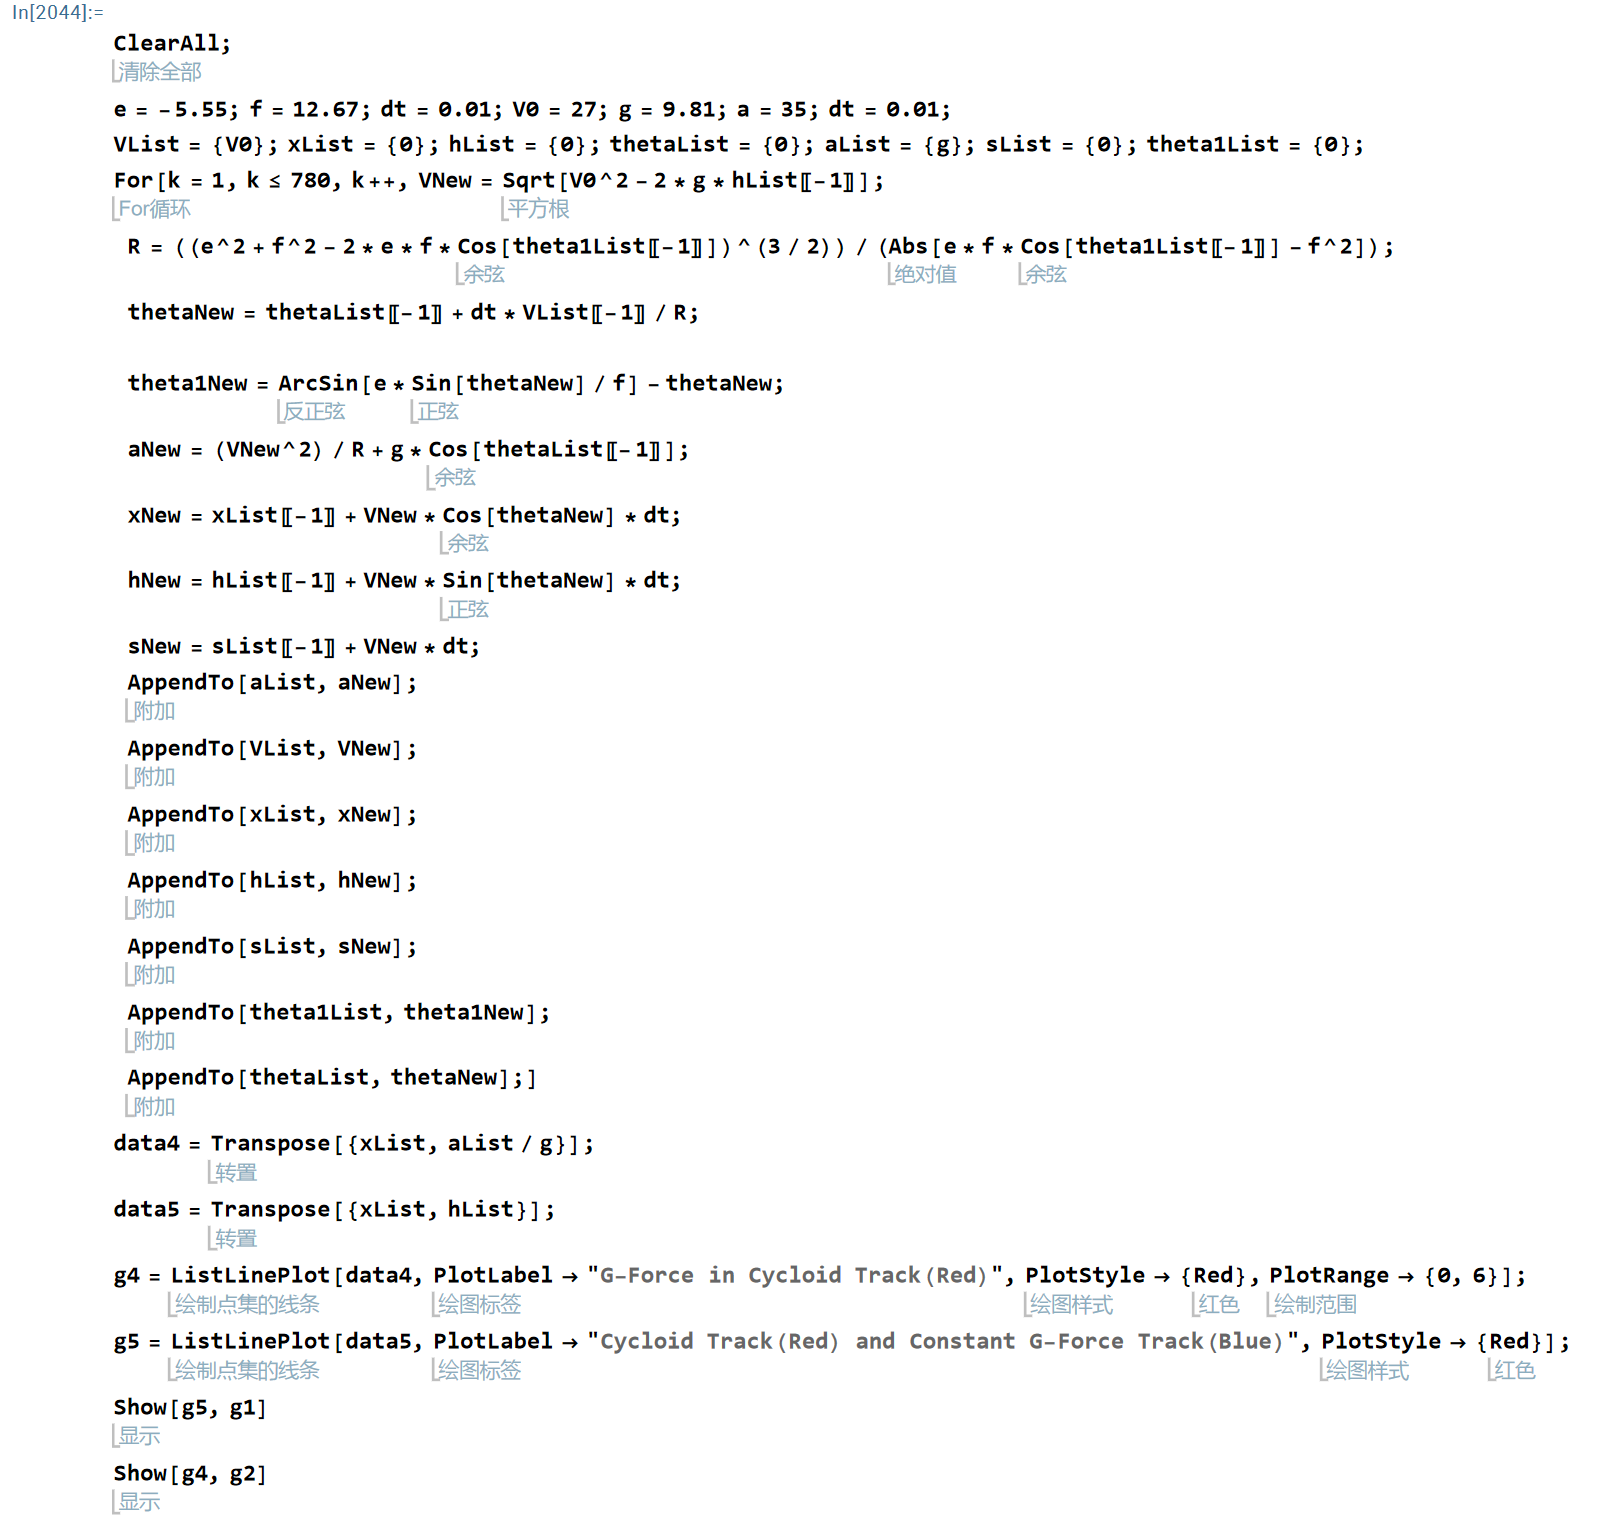
\includegraphics[width=0.6\textwidth]{8.png}
    \caption{Codes of Generating The Cycloid Track Shape (Non-friction)}
    \end{figure}  


The result follows:

\begin{figure}[H]
    \centering
    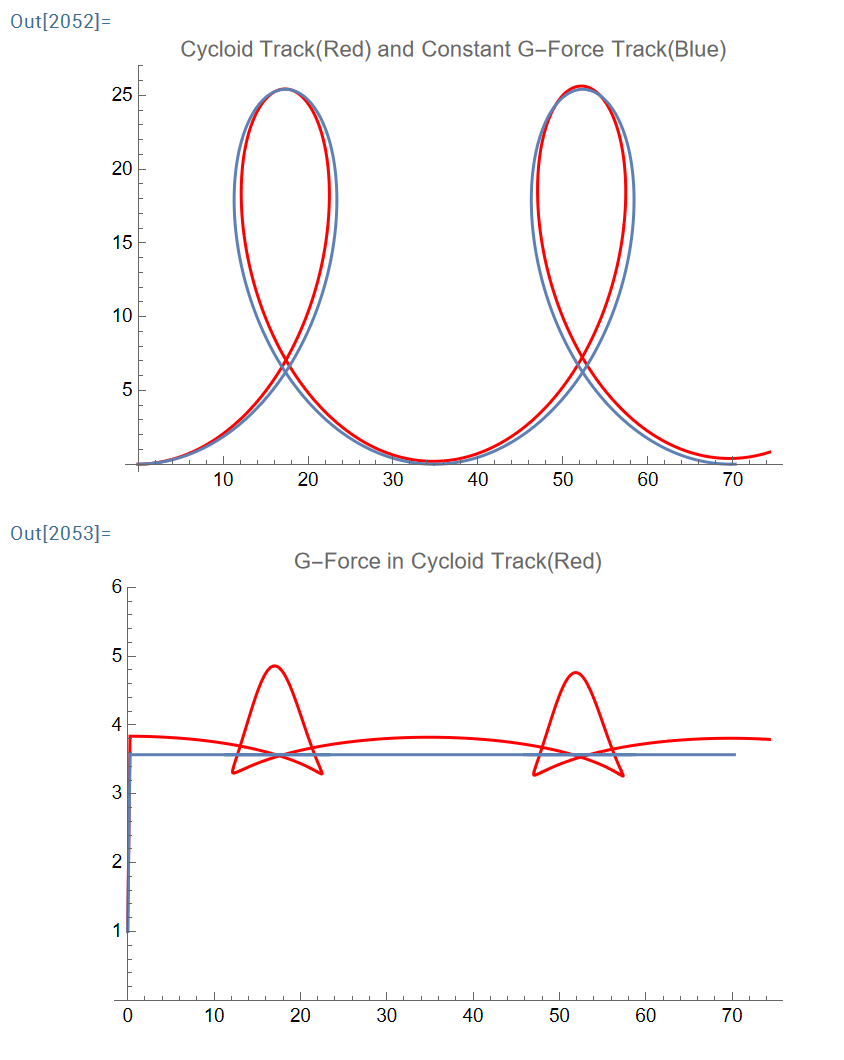
\includegraphics[width=0.4\textwidth]{9.png}
    \caption{The Cycloid Track Shape (Non-friction) and The G-force in Process}
    \end{figure}  

We can see that though the shape of cycloid is very similar to the one of constant G-force track, the G-force in the cycloid track at the peak is nearly $30\%$ larger than the constant G-force in our model. Meanwhile, the sudden change in G-force is unavoidable for both constant G-force track and cycloid track. This brings us back to the clothoid track, which provides a smooth change in G-force in the process.
\end{homeworkProblem}

\renewcommand{\currentSectionName}{Exploration}
\startSectionHeader{\currentSectionName}
\pagebreak
\begin{homeworkProblem}

For Möbius curve,(a roller coaster like Möbius curve)

$$\varphi (t)=
    \left(\begin{array}{cccc}
            (R+S\cos \frac{t}{2} )cost \\
            (R+S\cos \frac{t}{2})sint  \\
            S\sin(\frac{t}{2})
        \end{array}\right)
    ,t\in (0,4\pi ]
$$

Using mathematica to plot the curve and calculate the curavature $\kappa$ with t.

supposing no friction:

\

$\frac{1}{2}mv_{0}^{2}=\frac{1}{2}mv^{2}+\sin(\frac{t}{2})mg  $

\

$G-forces=\frac{v^{2}\kappa}{g}=\frac{(v_{0}^{2}-2\sin(\frac{t}{2})g)\kappa}{g}$

\

Let R=40, S=10, which means a fall of 20 meters, a radius at about 40 meters, with speed of 72 km/h, const speed


\begin{figure}[H]
    \centering
    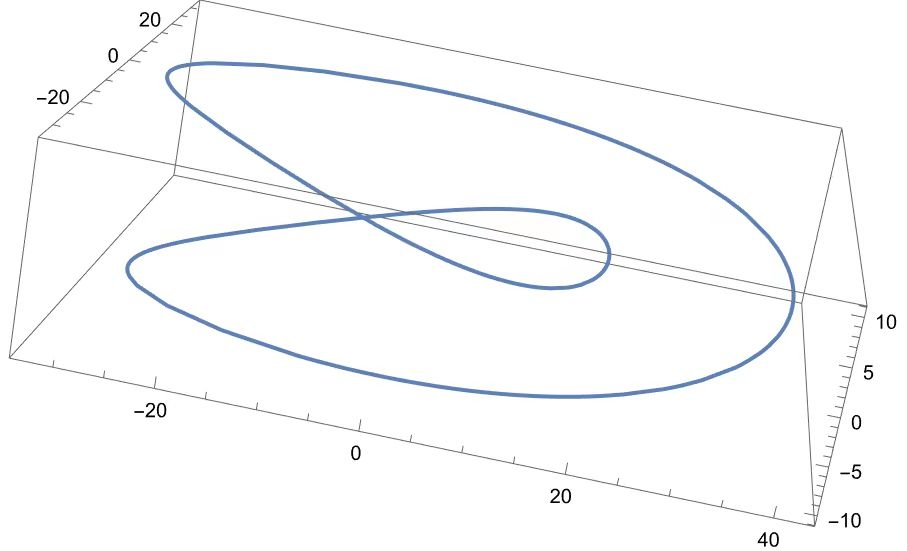
\includegraphics[width=0.4\textwidth]{p5-1.jpg}
\end{figure}
Having g force like
\begin{figure}[H]
    \centering
    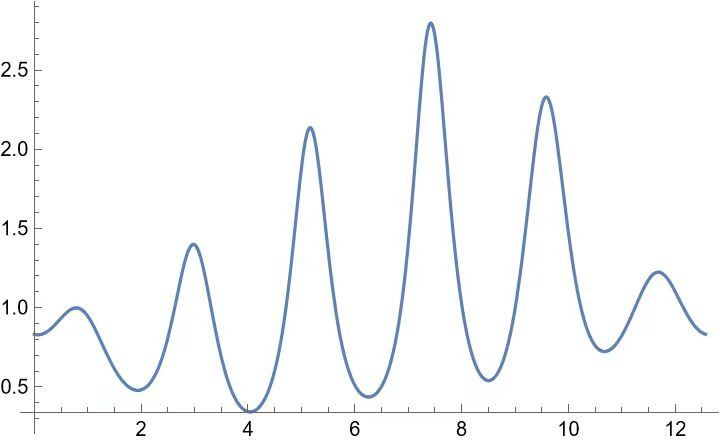
\includegraphics[width=0.4\textwidth]{p5-2.jpg}
\end{figure}

the change of accelerator is very large, which means people may enjoy themselve very much,but the value of acceleration is not very large , which means it is safe and will not cause injury.
\end{homeworkProblem}

\renewcommand{\currentSectionName}{References}
\startSectionHeader{\currentSectionName}
\pagebreak
\begin{thebibliography}{99}  
\addcontentsline{toc}{section}{References}

\bibitem{ref1} G. Birchak. Physics of the flip flap rollercoaster. https://mathsciencehistory.com/2020/01/19/physics-ofthe-flip-flap-rollercoaster/, 2020. Web. Accessed July 8th, 2022.

\bibitem{ref2} K. Brey. Geek challenge: Constant g-force coaster loops. https://www.dmcinfo.com/latestthink-ing/blog/id/228/geek-challenge-constant-g-force-coaster-loops, 2010. Web. Accessed July 8th, 2022.

\bibitem{ref3} A.-M. Pendrill. Kanonen (Photo 14/31). Roller Coaster database: https://rcdb.com/2905.htm\#p=12169,
2005. Web. Accessed July 8th, 2022.

\bibitem{ref4} A.-M. Pendrill. Rollercoaster loop shapes. Physics Education, 40(6):517–521, 2005.
https://doi.org/1-0.1088/0031-9120/40/6/001.

\bibitem{ref5} J. A. Rogers. Great American Scream Machine. CoasterGallery.com:
https://www.coastergall-ery.com/1999/GA25.html, 199. Web. Accessed July 8th, 2022.
\end{thebibliography}

\end{document}